\documentclass[a4paper]{article}
\usepackage{asymptote}
\usepackage{amsmath, enumitem, graphicx, geometry, tikz}
\usepackage[normalem]{ulem}
\geometry{margin=.4in}
\usetikzlibrary{intersections,angles,quotes,decorations.markings}
\begin{document}

\begin{center}
{\Large\bfseries January Block Day Round 1}\\[0.25cm]
{\large 28 January, 2026}\\[1cm]
\end{center}

\section*{Warmup}
\begin{enumerate}[itemsep=2cm]
    \item Darth Vader has grown his empire and now has 5 death stars. If each death star has 1,234 storm troopers and each storm trooper steals 2 light sabers, how many light sabers were stolen in total? \\
    \textbf{Solution: } The total number of storm troopers are $5\cdot1234$, and each storm trooper steals two light sabers. Thus, $5\cdot1234\cdot2=\boxed{12340}$ light sabers are stolen in total. \\
    \item On Wall Street, there is a company named Mapple. They sell Myphones and Mypads. Their company was worth \$10B and was distributed in 1 million different stocks. Meve Mobs owned one-eight of the shares. On Oct 31, the stocks went up 10\% and then down 10\% what was the dollar total Meve Mobs held after the scary halloween? \\
    \textbf{Solution: } Suppose a person has $x$ dollars. When the amount of money they have increases by $10\%$, the $x$ dollars rises to $1.1x$ dollars. When the $1.1x$ dollars decreases by $10\%$, $90\%$ is left, so there is $90\%\cdot1.1x=0.99x$ dollars. Since Meve Mobs has one eighth of the shares, he has $10,000,000,000/8=1,250,000,000$ dollars. Thus at the end he has $0.99\cdot 1,250,000,000=\boxed{1,237,500,000}$.
    \item Rebanto the Rhetorical Responder overloaded his schedule. He was only able to sleep 3 hours each school night and 5 hours all other nights. If a person sleeps less than 1500 hours a year they are considered a robot. If there are 180 days of school, how many hours of sleep does Rebanto get each year and is Rebanto a robot?  \\
    \textbf{Solution: } The number of hours of sleep total Rebanto gets only on school days is $180\cdot3$, and the number of hours of sleep total not on school days is $(365-180)\cdot5$. Thus, the total number of hours he sleeps in the whole year is $180\cdot3+(365-180)\cdot5=\boxed{1465}$ hours. Since this is less that $1500$ hours, Rebanto is a robot.
    \item Nitesh Kamanuru Purushotam loves to eat Kaju Katli (\textit{rhombus-shaped} dessert), and wants to create a Kaju Katli of his own. This morning, he measured the diagonals of the Kaju Katli. He measured $12$ and $14$ $\rm cm$. Please help Nitesh make a Kaju Katli by finding the side length of the rhombus (note the diagram is not drawn proportionally).
    
    \vspace{0.5cm}
    \begin{center}
        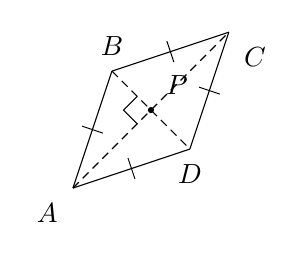
\begin{tikzpicture}[xscale=0.7, yscale=0.7, rotate=45]
          % vertices
          \coordinate (A) at (0,0);
          \coordinate (B) at (2,1);
          \coordinate (C) at (4,0);
          \coordinate (D) at (2,-1);
        
          % rhombus edges with single tick marks indicating equal sides
          \begin{scope}[
            decoration={markings, mark=at position 0.5 with {\draw[line width=0.35pt] (0,0.14) -- (0,-0.14);}}
          ]
            \draw[postaction=decorate] (A) -- (B);
            \draw[postaction=decorate] (B) -- (C);
            \draw[postaction=decorate] (C) -- (D);
            \draw[postaction=decorate] (D) -- (A);
          \end{scope}
        
          % diagonals (name paths for intersection)
          \path[name path=AC] (A) -- (C);
          \path[name path=BD] (B) -- (D);
        
          % compute intersection P of AC and BD
          \path[name intersections={of=AC and BD, by=P}];
        
          % draw diagonals (dashed)
          \draw[densely dashed] (A) -- (C);
          \draw[densely dashed] (B) -- (D);
        
          % right-angle marker at P between the two diagonals
          % (use A--P--B since A is on AC and B is on BD; angle APB = 90° in a rhombus)
          \pic [draw, line width=0.35pt, angle radius=7pt] {right angle = A--P--B};
        
          % mark and label P
          \fill (P) circle (1.6pt);
          \node[above right=2pt] at (P) {$P$};
        
          % vertex labels
          \node[below left=2pt]  at (A) {$A$};
          \node[above=2pt]       at (B) {$B$};
          \node[below right=2pt] at (C) {$C$};
          \node[below=2pt]       at (D) {$D$};
        \end{tikzpicture}
    \end{center}
    Drawing the diagonals. Label the rhombus as ABCD. Drawing the diagonals, they intersect at a right angle. Let the intersection point be $P$. Note that $P$ is the midpoint of both diagonals, so $BP=12/2=6$, and $CP=14/2=7$. Thus, the side length is $BC=\sqrt{BP^2+CP^2}=\sqrt{6^2+7^2}=\boxed{\sqrt{85}}$.
    \newpage
    \item (NO CALCULATOR) Marty \sout{McFly} Ho doesn't trust Doc Brown's latest version of the flux capacitor: he is skeptical of whether the DeLorean can reach 88 mph. He theorizes the DeLorean's velocity will follow a wonky cubic as follows. At what time $t$ is the DeLorean's velocity $v(t)$ equal to 88 mph?

    $$v(t) = 90t^3+6t^2-7t-1$$
    We need 
    \[v(t)=88\implies 90t^3+6t^2-7t-1=88\]
    \[\implies 90t^3+6t^2-7t-89\]
    By the rational root theorem, the roots of this polynomial should divide $89$, if they are integers. We first test $t=1$, which works, since it satisfies the equation. Thus, the answer is $t=\boxed{1}$.
    \end{enumerate}

    \newpage
    \section*{The Tale of \textit{Rohan The Rickety Racer}}
    
    Rohan the Rickety Racer returns home in his Volkswagen Tiguan, but on his way heu slipped onto the Circuit of the Americas (COTA) by destiny. Rohan joins the qualification matches. To his left, he sees Max Verstappen, and to his right, he sees Lewis Hamilton. They get on the track, but with a \textbf{twist}.
    
    
    \begin{enumerate}[itemsep=2.3cm]
    
    \item At time $t=0$, all three are on the track and drive at constant speeds.
    Rohan can complete $2$ laps in $5$ minutes, Max can complete $2$ laps in $3$ minutes, and Lewis can complete $1$ lap in $2$ minutes.
    \vspace{0.3cm}
    
    Rohan starts at the start/finish line. Max starts $\tfrac14$ of a lap \emph{ahead} of Rohan and drives in the \emph{same} direction as Rohan. Lewis starts $\tfrac14$ of a lap \emph{behind} Rohan, but drives in the \emph{opposite} direction. When is the first time all three racers are at the \emph{same point} on the track?
    
    \item At that time, where are they (describe the position as a fraction of a lap from the start/finish line)?

    \item After the qualification matches, Aarsh the Aston Martin Automobile Mechanic asks Rohan the Rickety Racer for his car keys to audit the Volkswagen Tiguan. However, little does Rohan know Aarsh has deeper intentions. In an ultimate act of deception, Aarsh drives away with Rohan's car on a $900$ m circular road. Rohan notices the theft exactly $45$ seconds after Aarsh leaves.
    \vspace{0.3cm}
    
    Aarsh drives at a constant speed of $27$ m/s, while Rohan chases him on foot at $9$ m/s. At what time (seconds) do Aarsh and Rohan meet?

    \item \textit{Flashback}: Lewis and Max race with all their might. Minutes before the race, Lewis bribes Aarsh to sabotage Rohan by stealing his car after the qualification matches. Knowing Aarsh has a success rate of 60\%, find the lowest success rate of another mechanic that Lewis should bribe to ensure that there is at least a 90\% chance that Rohan's car fails.

    \item Luckily, Rohan had a recipe to recreate a rejuvenating potion that grants him mighty strength: this allowed him to rescue the car and defeats the terrible Aarsh the Aston Martin Automobile Mechanic. However, Aarsh is quick to get back up: Speeding away, Rohan drives his car as fast as possible but accidentally runs into an orange traffic cone. Calculate the volume enclosed by the traffic cone assuming it is a truncated right cylinderical cone. 

    \begin{center}
    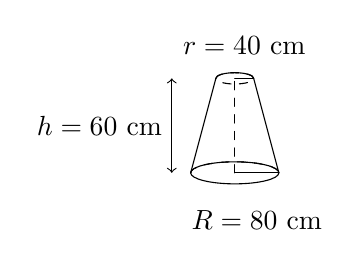
\begin{tikzpicture}[line cap=round, line join=round, scale=0.4]
    
    % geometry (drawing units, not cm)
    \def\h{3.0}      % picture height
    \def\aTop{0.6}   % top ellipse x-radius
    \def\bTop{0.18}  % top ellipse y-radius
    \def\aBot{1.4}   % bottom ellipse x-radius
    \def\bBot{0.35}  % bottom ellipse y-radius
    
    % key points
    \coordinate (TopC) at (0,\h);
    \coordinate (BotC) at (0,0);
    
    % side edges
    \draw (-\aTop,\h) -- (-\aBot,0);
    \draw ( \aTop,\h) -- ( \aBot,0);
    
    % top ellipse (front solid, back dashed)
    \draw (-\aTop,\h) arc[start angle=180,end angle=0, x radius=\aTop, y radius=\bTop];
    \draw[dashed] (\aTop,\h) arc[start angle=0,end angle=360, x radius=\aTop, y radius=\bTop];
    
    % bottom ellipse (front solid, back dashed)
    \draw[dashed] (-\aBot,0) arc[start angle=180,end angle=0, x radius=\aBot, y radius=\bBot];
    \draw (\aBot,0) arc[start angle=0,end angle=360, x radius=\aBot, y radius=\bBot];
    
    % radius markers
    \draw (TopC) -- ++(\aTop,0) node[midway, above, yshift=5pt] {$r=40\text{ cm}$};
    \draw (BotC) -- ++(\aBot,0) node[midway, below, yshift=-10pt] {$R=80\text{ cm}$};
    
    % height marker (dashed with double arrow)
    \draw[dashed] (BotC) -- (TopC);
    \draw[<->] (-2.0,0) -- (-2.0,\h) node[midway, left] {$h=60\text{ cm}$};
    
    \end{tikzpicture}
    \end{center}



\end{enumerate}

\end{document}
